\documentclass{article}
\usepackage[final]{neurips_2024}

\usepackage[utf8]{inputenc}
\usepackage[T1]{fontenc}
\usepackage{hyperref}
\usepackage{url}
\usepackage{booktabs}
\usepackage{amsfonts}
\usepackage{nicefrac}
\usepackage{microtype}
\usepackage{xcolor}
\usepackage{graphicx}
\usepackage{amsmath}
\usepackage{subcaption}

\title{Routing Visual Evidence: A Mixture of Connectors for Grounded Multimodal Reasoning}

\author{%
  Abdul Hafeez \\
  Lahore University of Management Sciences \\
  \texttt{25280098@lums.edu.pk} \\
  \And
  Verda Batool \\
  Lahore University of Management Sciences \\
  \texttt{24280065@lums.edu.pk} \\
  \And
  Shumaila Javed \\
  Lahore University of Management Sciences \\
  \texttt{24280078@lums.edu.pk} \\
  \And
  Muhammad Fasih Tariq \\
  Lahore University of Management Sciences \\
  \texttt{25280026@lums.edu.pk} \\
}

\begin{document}

\maketitle

\begin{abstract}
Multimodal large language models project all visual patches through a single, question-agnostic connector, leaving the language model to determine which visual evidence matters. We propose the \emph{Mixture of Connectors} (MoC), built on LLaVA-1.5-7B~\citep{liu2024llava}, which routes each sample to one of four structurally distinct connector experts based on the question. Our key contribution is the \emph{Question-Conditioned Gating Projector} (QCGP, $E_4$), which gates each patch using cosine similarity between the question and patch tokens. A two-layer router selects one expert per sample, trained with a Switch Transformer load-balancing loss~\citep{fedus2022switch}. On ScienceQA's image-only split~\citep{lu2022scienceqa}, MoC reaches 73.8\% validation accuracy at epoch 2 with balanced routing ($E_1$: 30.5\%, $E_2$: 20.5\%, $E_3$: 28.4\%, $E_4$: 20.6\%). However, single-expert ablations reveal that randomly initialized experts ($E_2$--$E_4$) reach only 34--39\% individually, far below $E_1$'s 65.6\% from its pretrained projector. Since all experts converge to similar training loss ($\approx$1.90--1.93), this 30-point gap shows that pretrained initialization, not architecture, dominates at our 6{,}218-sample data budget. Training past epoch 2 degrades MoC to 62.2\% with $\Delta_v$ inverting to $-8.0\%$, making early stopping essential. The QCGP temperature $\tau_g$ shifts only $-0.0011$, producing near-uniform heatmaps. A failure analysis of 100 errors finds 48\% perception, 41\% reasoning, and 11\% chain-of-thought rescue---less perception-heavy than the 67\% reported for RLVR-trained models~\citep{wang2026papo}.

\end{abstract}

\section{Introduction}
\label{sec:intro}

In multimodal language models, the connector that maps visual patch embeddings into the language model's token space typically operates without knowledge of the question. Every patch is projected through the same fixed transformation, and the language model is left responsible for selecting which visual evidence matters for a given query. This question-blindness has measurable consequences: approximately 67\% of multimodal reasoning failures in recent reinforcement-learning-trained models trace to visual misperception rather than flawed inference~\citep{wang2026papo}.

Existing connectors each commit to a single point in the locality-versus-compression tradeoff, and none condition on the input query. LLaVA-1.5~\citep{liu2024llava} keeps all 576 patches via a question-blind two-layer MLP. InstructBLIP~\citep{dai2023instructblip} injects the question into a Q-Former and reaches 90.7\% on ScienceQA-IMG, but compresses patches to 32 slots, losing spatial detail. MoE-style connectors like CuMo~\citep{li2024cumo} and MoCHA~\citep{pang2026mocha} add routing but use identical FFN experts, while MoVA~\citep{zong2024mova} routes across multiple frozen encoders at high memory cost. As \citet{cha2024honeybee} show, the right balance between locality and compression likely depends on the question.

We address this with two architectural changes. First, the \emph{Question-Conditioned Gating Projector} (QCGP) projects each patch and the pooled question vector into a shared subspace, computes per-patch relevance scores via cosine similarity, and modulates the patch features with a learned sigmoid gate before the LLM projection. Unlike Q-Former-style compression, QCGP preserves the full 576-token sequence. Second, the \emph{Mixture of Connectors} (MoC) routes each sample through one of four structurally distinct experts: the frozen pretrained LLaVA MLP ($E_1$), a Q-Former ($E_2$), an attention-pooled global token ($E_3$), and QCGP ($E_4$). The router is a two-layer MLP that consumes only the question vector and is trained jointly with the experts under a Switch-Transformer load-balancing objective~\citep{fedus2022switch}.

Our experiments on the ScienceQA image-only split~\citep{lu2022scienceqa} yield three main findings. The full MoC reaches 73.8\% validation accuracy at epoch 2, comfortably exceeding any single expert, and the router maintains a balanced selection distribution without collapse. However, individually trained $E_2$, $E_3$, and $E_4$ reach only 34--39\% image accuracy because they start from random initialization, while $E_1$ inherits LLaVA's pretrained projector weights and attains 65.6\%. The QCGP temperature $\tau_g$ remains within 0.0011 of its initialization throughout training, and the corresponding patch-relevance heatmaps are visually flat, indicating that the 6{,}218-sample budget is insufficient for the gating mechanism to acquire selective behaviour. Together, these results suggest that in low-data regimes, warm-starting heterogeneous experts from a pretrained projector matters more than architectural novelty.

\section{Related Work}
\label{sec:relwork}

The connector $\phi\colon \mathbb{R}^{N \times d_v} \to \mathbb{R}^{L \times d}$, mapping $N$ frozen-encoder patch tokens into $L$ LLM-space embeddings, is the architectural axis that this work modifies. Three threads of prior research contextualize our contribution: foundational connector designs, query-conditioned visual feature extraction, and mixture-of-experts approaches in Vision-Language Models.

\paragraph{Foundational Connector Designs.}
\citet{radford2021clip} established the dual-encoder paradigm that produces the patch tokens our connectors consume; \citet{liang2022modgap} show that its contrastive objective induces a \emph{modality gap} that any downstream projector must bridge. \citet{liu2024llava} demonstrate that a two-layer MLP with GELU nonlinearity, applied identically to each patch, suffices for state-of-the-art ScienceQA accuracy. The alternative paradigm of learned-query compression, originating with \citet{alayrac2022flamingo}'s Perceiver Resampler and formalized by \citet{li2023blip2}'s Q-Former, reduces the visual-token budget but discards spatial structure. \citet{cha2024honeybee} characterize the resulting locality-versus-compression tradeoff and motivate projector designs that retain spatial detail.

\paragraph{Query-Conditioned Visual Feature Extraction.}
The aforementioned connectors are invariant to the input query $x^T$. \citet{ilievski2016fda} showed that question-driven region selection improves grounded VQA. InstructBLIP~\citep{dai2023instructblip} injects the question into Q-Former self-attention and reaches 90.7\% on ScienceQA-IMG, but the resulting features still compress to $K$ slots. Our QCGP ($E_4$) conditions on the question at full patch resolution using cosine-similarity gates (Section~\ref{sec:method}). \citet{zhang2025sail} and \citet{zou2026vlsa} further show that standard pretraining does not close the cross-modal alignment gap, motivating an explicit bridging mechanism.

\paragraph{Mixture of Experts in VLMs.}
\citet{shazeer2017moe} introduced sparsely-gated MoE; \citet{fedus2022switch} simplified it to top-1 routing with a load-balancing loss, which we adopt. MoE-LLaVA~\citep{lin2024moellava} places MoE inside the LLM's FFN layers, leaving the connector unchanged. CuMo~\citep{li2024cumo} and MoCHA~\citep{pang2026mocha} route at the connector level but use identical expert architectures. MoVA~\citep{zong2024mova} routes across frozen vision encoders at high memory cost. Our MoC instead uses a single CLIP encoder and routes across four \emph{structurally distinct} connectors ($E_1$--$E_4$).

\paragraph{Hallucination and the ScienceQA Benchmark.}
\citet{wang2026papo} find that approximately 67\% of errors in RLVR-trained MLLMs stem from visual misperception, consistent with the hallucination inequality $P_\theta(\text{ans} \mid x^T) \gg P_\theta(\text{ans} \mid x^V)$: the language prior overwrites visual evidence whenever the connector fails to ground query-relevant content. \citet{li2023pope} formalize the related problem of object hallucination with the POPE diagnostic protocol. ScienceQA~\citep{lu2022scienceqa} provides an image-required versus text-only split that supports our visual grounding gap metric $\Delta_v$ and the three-bucket failure analysis we adopt from \citet{zhang2023multimodalcot}.

\section{Methodology}
\label{sec:method}

\subsection{System Overview and Visual Grounding Gap}
\begin{figure}[h]
\centering
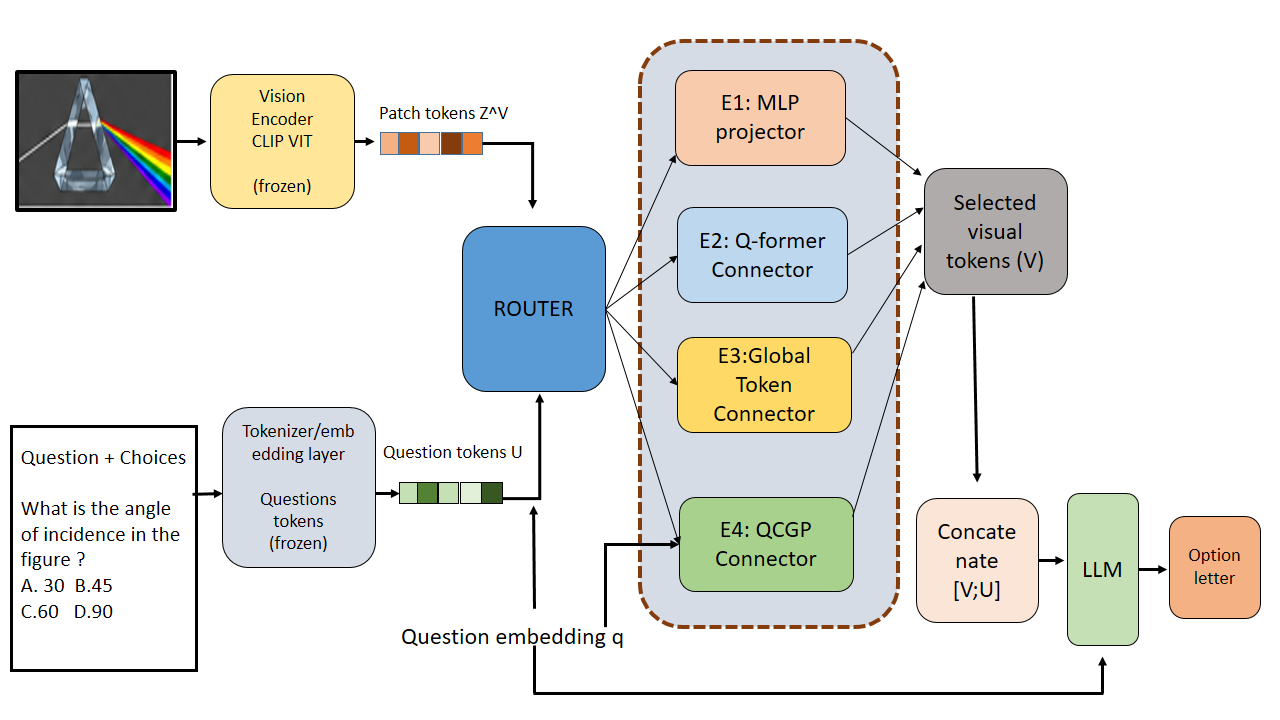
\includegraphics[width=0.9\linewidth]{architecture_diagram updated.png}
\caption{\textbf{Mixture of Connectors (MoC) architecture.} The image is encoded by a frozen CLIP ViT-L/14 into $N=576$ patch tokens $Z^V$. The question is embedded by a frozen tokenizer/embedding layer into tokens $U$, from which a question vector $\mathbf{q}$ is pooled. The question-conditioned router selects one of four connector experts: $E_1$ (pretrained LLaVA MLP, frozen, $L=576$), $E_2$ (Q-Former, 32 learned queries, $L=32$), $E_3$ (global attention-pooled token, $L=1$), or $E_4$ (QCGP, question-conditioned per-patch gating, $L=576$). The selected expert's output $\phi_k(Z^V)$ is concatenated with $U$ and fed into the LoRA-fine-tuned Vicuna-1.5-7B LLM to produce the predicted answer.}
\label{fig:arch}
\end{figure}

Figure~\ref{fig:arch} illustrates the full MoC pipeline. A frozen CLIP ViT-L/14 encodes the image at $336 \times 336$ resolution into $N=576$ patch tokens $Z^V \in \mathbb{R}^{N \times d_v}$ with $d_v=1024$. The question is tokenized and embedded by the LLM's frozen embedding layer into token embeddings $U \in \mathbb{R}^{T \times d}$ with $d=4096$. A learned attention pooling step extracts a single question vector $\mathbf{q} \in \mathbb{R}^d$, which drives both the router and the QCGP expert. The router selects one expert $k^*$, whose output $\phi_{k^*}(Z^V) \in \mathbb{R}^{L_{k^*} \times d}$ is concatenated with $U$ and fed to a 4-bit quantized Vicuna-1.5-7B with LoRA adapters on the attention projections. The LLM generates the answer as a single option letter.

To measure how strongly a model relies on visual evidence rather than language priors, we adopt the \emph{visual grounding gap}
\begin{equation*}
    \Delta_v = \text{Acc}_{\text{image}} - \text{Acc}_{\text{text-only}},
\end{equation*}
where $\text{Acc}_{\text{text-only}}$ is the same model evaluated with the \texttt{<image>} token removed and no image tensor supplied. Larger $\Delta_v$ values indicate that accuracy depends genuinely on visual evidence rather than on language shortcuts.

\subsection{Mixture of Connectors}
\label{sec:method-moc}

The MoC replaces the single MLP projector with four parallel experts and a router that selects one per sample. Before routing, the question vector $\mathbf{q}$ is extracted from the LLM token embeddings $U$ via attention pooling with a learned query $\mathbf{q}_{\text{pool}} \in \mathbb{R}^d$
\begin{equation*}
    \mathbf{q} = \mathrm{softmax}\!\left(\frac{\mathbf{q}_{\text{pool}}^\top U^\top}{\sqrt{d}}\right) U \in \mathbb{R}^{d}.
\end{equation*}
This single vector summarises the question and is shared between the router and $E_4$. Each expert $k$ maps $\phi_k\colon Z^V \mapsto V^{(k)} \in \mathbb{R}^{L_k \times d}$, spanning different points on the locality-versus-compression axis.

\textbf{$E_1$ (Pretrained MLP, $L_1 = 576$).} The first expert is LLaVA's original two-layer MLP projector, held frozen: $\phi_1(z_i^V) = W_2 \sigma(W_1 z_i^V)$ with $\sigma=\text{GELU}$. It introduces no new trainable parameters and serves as a strong reference because of its pretrained initialization on millions of image-text pairs.

\textbf{$E_2$ (Q-Former, $L_2 = 32$).} The second expert applies BLIP-2-style cross-attention compression~\citep{li2023blip2}. $K=32$ learnable query vectors $Q \in \mathbb{R}^{K \times d}$ attend over the patch sequence,
\begin{equation*}
    \phi_2(Z^V) = \mathrm{softmax}\!\left(\frac{Q K_v^\top}{\sqrt{d}}\right) V_v, \quad K_v = Z^V W_K, \quad V_v = Z^V W_V,
\end{equation*}
with $W_K, W_V \in \mathbb{R}^{d_v \times d}$ (8{,}519{,}680 trainable parameters). The output sequence is bounded by $L_2 = K \ll N$, which improves efficiency but irreversibly discards fine spatial structure.

\textbf{$E_3$ (Global Token, $L_3 = 1$).} The third expert collapses the full image to a single token by attention pooling along the patch dimension,
\begin{equation*}
    \phi_3(Z^V) = W_{E_3} \sum_{i=1}^{N} \mathrm{softmax}_i\!\left(\frac{\mathbf{w}^\top z_i^V}{\sqrt{d_v}}\right) z_i^V,
\end{equation*}
with $\mathbf{w} \in \mathbb{R}^{d_v}$ and $W_{E_3} \in \mathbb{R}^{d \times d_v}$ (4{,}199{,}424 trainable parameters). It is the cheapest expert and the strongest single point of compression, trading almost all spatial information for a single summary vector.

\textbf{$E_4$ (QCGP, $L_4 = 576$).} QCGP computes a per-patch relevance score from the question vector, gates each patch's channels by that score, and projects the result into LLM space while preserving spatial resolution. To bridge the geometric modality gap~\citep{liang2022modgap}, both the question vector and each patch token are projected to a shared $d_k = 256$ subspace and $L_2$-normalised
\begin{align}
  \hat{u} &= \tfrac{W_q \mathbf{q}}{\|W_q \mathbf{q}\|_2}, \quad
  \hat{k}_i = \tfrac{W_k z_i^V}{\|W_k z_i^V\|_2}, \quad
  \alpha_i = \mathrm{softmax}_i\!\left(\frac{\hat{u}^\top \hat{k}_i}{\tau_g}\right), \nonumber\\
  \mathbf{g}_i &= \sigma\!\left(\alpha_i W_g + \mathbf{b}_g\right), \quad
  \phi_4(Z^V)_i = W_{E_4}\!\left(z_i^V \odot \mathbf{g}_i\right),
  \label{eq:qcgp}
\end{align}
where $W_q \in \mathbb{R}^{d_k \times d}$, $W_k \in \mathbb{R}^{d_k \times d_v}$, $W_g \in \mathbb{R}^{d_v}$, $\mathbf{b}_g \in \mathbb{R}^{d_v}$, $W_{E_4} \in \mathbb{R}^{d \times d_v}$, $\sigma$ is the sigmoid, and $\tau_g$ is a learnable temperature initialised to 1.0. The scalar $\alpha_i$ expands to a per-channel gate $\mathbf{g}_i$ via $W_g$, letting the model suppress channels based on question-patch alignment. QCGP retains all 576 tokens ($L_4 = N$) with 5{,}511{,}169 trainable parameters.

The \textbf{router} is a two-layer MLP that consumes $\mathbf{q}$ and emits a softmax distribution over the four experts:
\begin{equation}
  \mathbf{r} = \mathrm{softmax}\!\left(W_r^{(2)}\,\mathrm{GELU}\!\left(W_r^{(1)} \mathbf{q}\right)\right) \in \mathbb{R}^4,
  \qquad k^* = \arg\max_k r_k,
  \label{eq:router}
\end{equation}
with $W_r^{(1)} \in \mathbb{R}^{d_r \times d}$, $W_r^{(2)} \in \mathbb{R}^{4 \times d_r}$, and $d_r = 64$. $W_r^{(2)}$ is initialised to zero so the router begins with a uniform $r_k = 0.25$ across experts, preventing early collapse. Discrete top-1 selection is non-differentiable; we use a straight-through estimator so gradients update the router weights through $\mathbf{r}$. To prevent the router from converging to a single expert, we add the Switch Transformer auxiliary loss~\citep{fedus2022switch}:
\begin{equation}
  \mathcal{L}_{\text{lb}} = K \sum_{k=1}^{K} f_k\, p_k,
  \qquad
  \mathcal{L} = \mathcal{L}_{\text{CE}} + \lambda_{\text{lb}}\, \mathcal{L}_{\text{lb}},
  \label{eq:lb}
\end{equation}
where $f_k$ is the fraction of the batch dispatched to expert $k$ (computed from the argmax, no gradient) and $p_k$ is the mean router probability for expert $k$ (with gradient). The product $f_k\,p_k$ grows when the router concentrates mass on one expert, which raises the loss and forces redistribution.

\subsection{QLoRA Fine-Tuning Setup}

Memory constraints on a single A100 preclude full fine-tuning of the 7B backbone. We use QLoRA~\citep{dettmers2023qlora}: the LLM is quantized to 4-bit NF4 precision via \texttt{bitsandbytes}, and LoRA adapters are added to the four attention projection layers (\texttt{q\_proj}, \texttt{k\_proj}, \texttt{v\_proj}, \texttt{o\_proj}). The CLIP encoder, the original MLP projector ($E_1$), and the output head remain frozen. Following the QLoRA recipe, \texttt{prepare\_model\_for\_kbit\_training} is called before \texttt{get\_peft\_model}; this ordering ensures gradient checkpointing is compatible with the quantized weights and that 1D parameters are upcast to float32 for numerical stability. The new connector experts ($E_2$, $E_3$, $E_4$), the router, and the question pooler are kept in float32 to avoid softmax overflow; their forward methods cast inputs to the local weight dtype and return outputs in the caller's dtype, allowing seamless interoperation with the float16 vision pipeline. Two parameter groups are used: connector experts and the router at $2 \times 10^{-4}$, and LoRA adapters at $5 \times 10^{-5}$. Table~\ref{tab:hparams} reports the full configuration.

\begin{table}[h]
\centering
\caption{\textbf{QLoRA fine-tuning hyperparameters.} Two parameter groups: connector experts and router at $2{\times}10^{-4}$; LoRA adapters at $5{\times}10^{-5}$.}
\label{tab:hparams}
\small
\begin{tabular}{lc@{\hspace{2em}}lc}
\toprule
\textbf{Hyperparameter} & \textbf{Value} & \textbf{Hyperparameter} & \textbf{Value} \\
\midrule
Quantization                         & 4-bit NF4 & LR (LoRA adapters)           & $5\times10^{-5}$ \\
LoRA rank $r$                        & 16        & Scheduler                    & Cosine, 3\% warmup \\
LoRA $\alpha$                        & 32        & Effective batch size         & 16 (4 $\times$ 4 accum.) \\
LoRA dropout                         & 0.05      & Training samples             & 6{,}218 (image-only train) \\
LoRA targets                         & q/k/v/o\_proj & Max sequence length      & 512 \\
LR (connectors + router)             & $2\times10^{-4}$ & Optimizer              & AdamW \\
Load-balancing weight $\lambda_{\text{lb}}$ & 0.01 & $d_r$ (router hidden)       & 64 \\
$d_k$ (QCGP subspace)                & 256       & $K$ (Q-Former queries)       & 32 \\
\bottomrule
\end{tabular}
\end{table}

\section{Experimental Design}

\subsection{Research Questions}

The experimental program is organised around three research questions. \textbf{RQ1}: Does moving from the midterm's 2{,}000-sample LoRA fine-tuning to the full 6{,}218-sample QLoRA setup improve accuracy and visual grounding? \textbf{RQ2}: When trained in isolation, can connectors initialised from random weights ($E_2$, $E_3$, $E_4$) match the pretrained MLP projector ($E_1$)? \textbf{RQ3}: Does combining all four experts under a learned router yield accuracy that exceeds any single expert?

\subsection{Dataset, Evaluation, and Baselines}

We use ScienceQA (\texttt{derek-thomas/ScienceQA} on HuggingFace) restricted to questions with associated images, yielding 6{,}218 training, 2{,}097 validation, and 2{,}017 test samples. The single-expert ablations evaluate each model on a 500-sample subset of the test split for tractable comparison across four configurations. The MoC training run evaluates on a 200-sample validation subset every 750 steps to select the best checkpoint, and on a 500-sample test subset at the end of training. Subject-level analysis and the failure-case audit (Section~\ref{sec:failure}) use the full 2{,}017-sample test split with the deployed $E_1$ model. Answer extraction is performed by a regex cascade that handles parenthesised letters, ``the answer is X'' phrases, and standalone capitals. Midterm baselines (zero-shot and 2{,}000-sample LoRA) were run on an RTX 5080; all QLoRA training and the Part-E analyses were performed on a single A100 (Google Colab). The midterm zero-shot LLaVA-1.5-7B and the 2{,}000-sample LoRA-tuned model serve as the primary baselines for RQ1.

\section{Results and Findings}

\subsection{Main Comparison}

Table~\ref{tab:full} reports accuracies and visual grounding gaps across all configurations. The midterm baselines establish that zero-shot LLaVA-1.5-7B achieves 63.5\% image accuracy with $\Delta_v = +7.5\%$, and that LoRA fine-tuning on 2{,}000 samples leaves image accuracy nearly unchanged (62.6\%) while reducing text-only accuracy from 56.0\% to 51.0\%. The resulting widened gap of $\Delta_v = +11.6\%$ confirms the midterm prediction: the question-blind projector does not improve top-line accuracy, but minimal domain adaptation does sharpen the model's reliance on visual evidence.

The full QLoRA results address RQ2 and RQ3 directly. On the 500-sample ablation subset, $E_1$ achieves 65.6\% image accuracy with $\Delta_v = +27.4\%$, while $E_2$, $E_3$, and $E_4$ reach 34.0\%, 39.0\%, and 35.5\% respectively. The 30-point margin between $E_1$ and the random-init experts is not attributable to optimisation failure: all four experts converge to similar final training loss (1.90--1.93 at step 750). The gap reflects initialisation. $E_1$ inherits the LLaVA projector trained on millions of image-text pairs, whereas $E_2$, $E_3$, and $E_4$ are trained from scratch on 6{,}218 samples. $E_4$ shows a distinctive within-group pattern: its text-only accuracy (13.0\%) is the lowest of any configuration, yielding $\Delta_v = +22.5\%$. The QCGP gate is therefore suppressing language shortcuts, although it has not yet learned to surface correct visual evidence in their place. Re-evaluating $E_1$ on the full 2{,}017-sample test split yields 65.5\% image and 60.6\% text accuracy ($\Delta_v = +5.0\%$); the smaller text-only $\Delta_v$ compared to the 500-sample subset reflects the broader text-answerable question distribution in the full split and is consistent with prior ScienceQA reports.

The full MoC achieves 73.8\% validation accuracy at step 750 (end of epoch 2), exceeding the strongest single expert by 8.2 percentage points. Continued training reverses this gain. At step 1{,}900 (end of epoch 5), image accuracy falls to 62.2\% and text-only accuracy rises to 70.2\%, inverting $\Delta_v$ to $-8.0\%$. The architecture is viable, but peak performance is reached early and erodes thereafter; validation-based early stopping is required for any extension of this work.

\begin{table}[h]
\centering
\caption{\textbf{Complete results on the ScienceQA image-only test set.} Single-expert QLoRA configurations are evaluated on a 500-sample subset; MoC checkpoints are evaluated on a 200-sample validation subset (best) and a 500-sample test subset (final). The bottom row reports $E_1$ re-evaluated on the full 2{,}017-sample test split, which is the basis for the subject-level and failure-bucket analyses in Section~\ref{sec:failure}.}
\label{tab:full}
\small
\begin{tabular}{lccc}
\toprule
\textbf{Model} & \textbf{Image Acc.} & \textbf{Text Acc.} & $\Delta_v$ \\
\midrule
Zero-shot LLaVA-1.5-7B (midterm, $n=200$)         & 63.5\% & 56.0\% & $+$7.5\%  \\
LoRA $E_1$, 2k samples (midterm)                  & 62.6\% & 51.0\% & $+$11.6\% \\
\midrule
QLoRA $E_1$ (pretrained projector, $n=500$)       & \textbf{65.6\%} & 38.2\% & $+$27.4\% \\
QLoRA $E_2$ (Q-Former, $n=500$)                   & 34.0\% & 33.0\% & $+$1.0\%  \\
QLoRA $E_3$ (global token, $n=500$)               & 39.0\% & 33.5\% & $+$5.5\%  \\
QLoRA $E_4$ (QCGP, $n=500$)                       & 35.5\% & 13.0\% & $+$22.5\% \\
\midrule
MoC best val (step 750, epoch 2, $n=200$)         & \textbf{73.8\%} & 71.8\% & $+$2.0\%  \\
MoC final (step 1{,}900, epoch 5, $n=500$)        & 62.2\% & 70.2\% & $-$8.0\%  \\
\midrule
QLoRA $E_1$, full test split ($n=2{,}017$)        & 65.5\% & 60.6\% & $+$5.0\%  \\
\bottomrule
\end{tabular}
\end{table}

\subsection{Router Behaviour}

The router maintains a balanced distribution across all four experts throughout training. Figure~\ref{fig:router} reports the cumulative selection counts over the 1{,}900-step run (30{,}440 routing decisions): $E_1$ at 30.5\%, $E_2$ at 20.5\%, $E_3$ at 28.4\%, $E_4$ at 20.6\%. The maximum gap between the most- and least-selected experts is 10.1 percentage points, well below the threshold that would indicate routing collapse. $E_1$ and $E_3$ are slightly preferred, consistent with $E_1$'s superior individual accuracy and $E_3$'s low compute cost. The load-balancing loss therefore achieves its primary goal of preventing single-expert dominance. Whether the router's selections are input-dependent or approximately random cannot be determined from cumulative training-time counts, as the router weights were not saved with the LoRA checkpoint, preventing a post-hoc test-set analysis.

\subsection{QCGP Gate Heatmaps and $\tau_g$ Convergence}

Figure~\ref{fig:heatmaps} visualises the per-patch relevance scores $\alpha_i$ produced by $E_4$ on four ScienceQA questions: three spatially grounded queries and one general counter-example. Each $\alpha \in \mathbb{R}^{576}$ vector is reshaped to the $24 \times 24$ CLIP patch grid and overlaid on the source image. Peak $\alpha$ values across the dataset range from 0.00199 to 0.00209, compared to the uniform baseline of $1/576 \approx 0.00174$, so the most-attended patches are only 15--19\% above uniform. The spatial questions and the counter-example produce visually indistinguishable maps, indicating that QCGP has not learned to differentiate question types.

Figure~\ref{fig:taug} tracks the learnable temperature $\tau_g$ over training. $\tau_g$ moves from 0.9996 to 0.9985, a net change of $-0.0011$, and stabilises well before training ends. Smaller $\tau_g$ values would sharpen the softmax in Eq.~\ref{eq:qcgp} and concentrate attention on fewer patches; larger values would diffuse it. The near-zero net movement implies that the cross-entropy objective on 6{,}218 samples does not provide enough signal to push $\tau_g$ off its initialisation, which directly explains the flat heatmaps. Section~\ref{sec:disc} returns to this finding and its implications.

\begin{figure}[h]
\centering
\begin{subfigure}[b]{0.30\linewidth}
  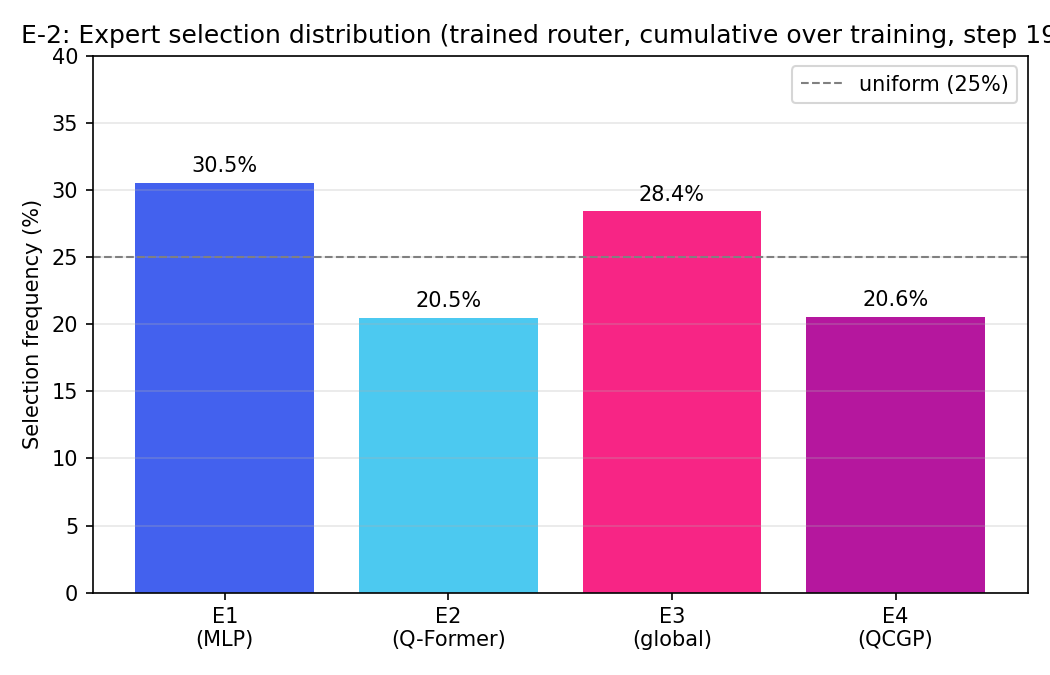
\includegraphics[width=\linewidth]{router_distribution.png}
  \caption{Router selection frequencies.}
  \label{fig:router}
\end{subfigure}
\hfill
\begin{subfigure}[b]{0.32\linewidth}
  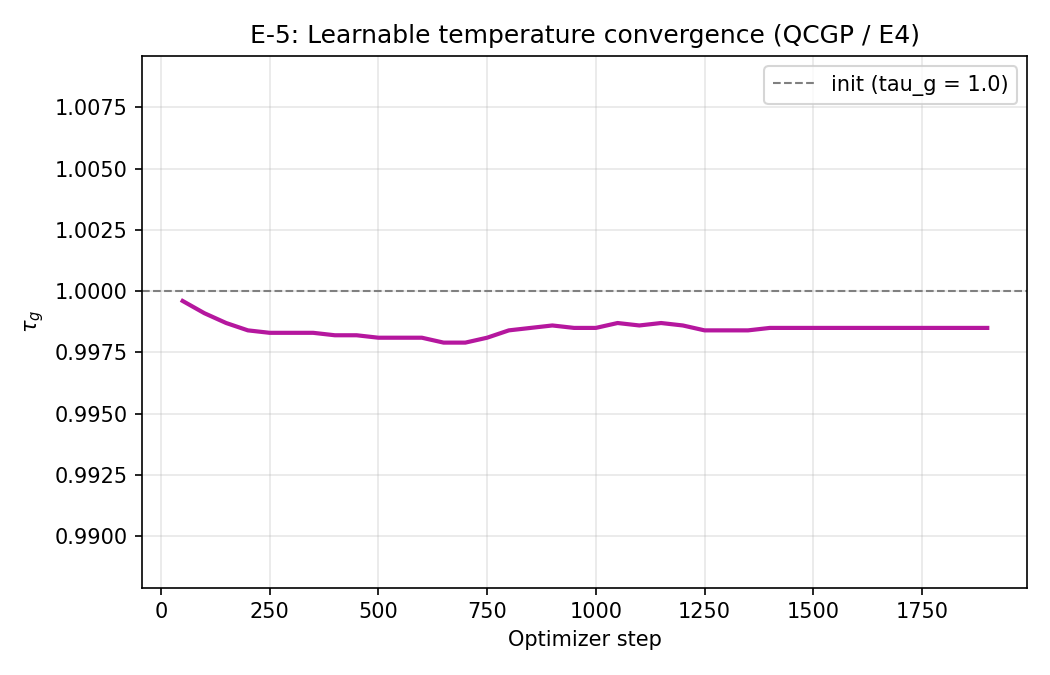
\includegraphics[width=\linewidth]{tau_g_convergence.png}
  \caption{$\tau_g$ across training steps.}
  \label{fig:taug}
\end{subfigure}
\hfill
\begin{subfigure}[b]{0.32\linewidth}
  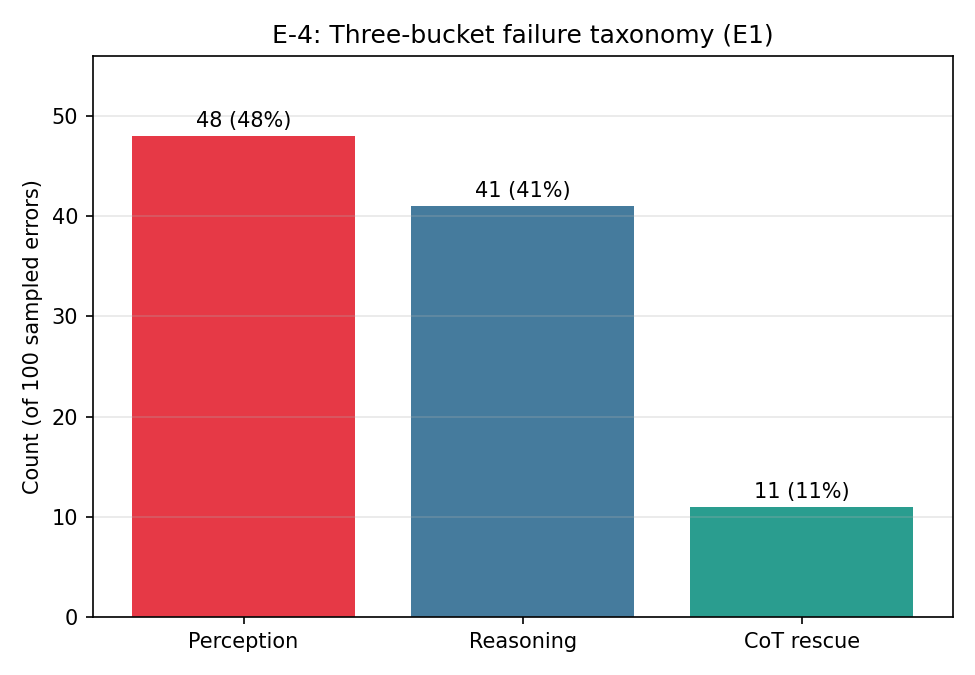
\includegraphics[width=\linewidth]{failure_buckets.png}
  \caption{Three-bucket failure analysis on $E_1$.}
  \label{fig:failure}
\end{subfigure}
\caption{\textbf{Aggregate analyses for the trained MoC.} (a) Cumulative router selections over 1{,}900 training steps (30{,}440 decisions) confirm the load-balancing loss prevents collapse. (b) Learnable temperature $\tau_g$ moves only $-0.0011$ across training, indicating near-neutral gating sharpness. (c) 100 randomly sampled $E_1$ errors (seed 42) classified as perception, reasoning, or chain-of-thought rescue; the PAPO~\citep{wang2026papo} 67\% perception baseline is shown for reference.}
\label{fig:agg}
\end{figure}

\begin{figure}[h]
\centering
\begin{subfigure}[b]{0.24\linewidth}
  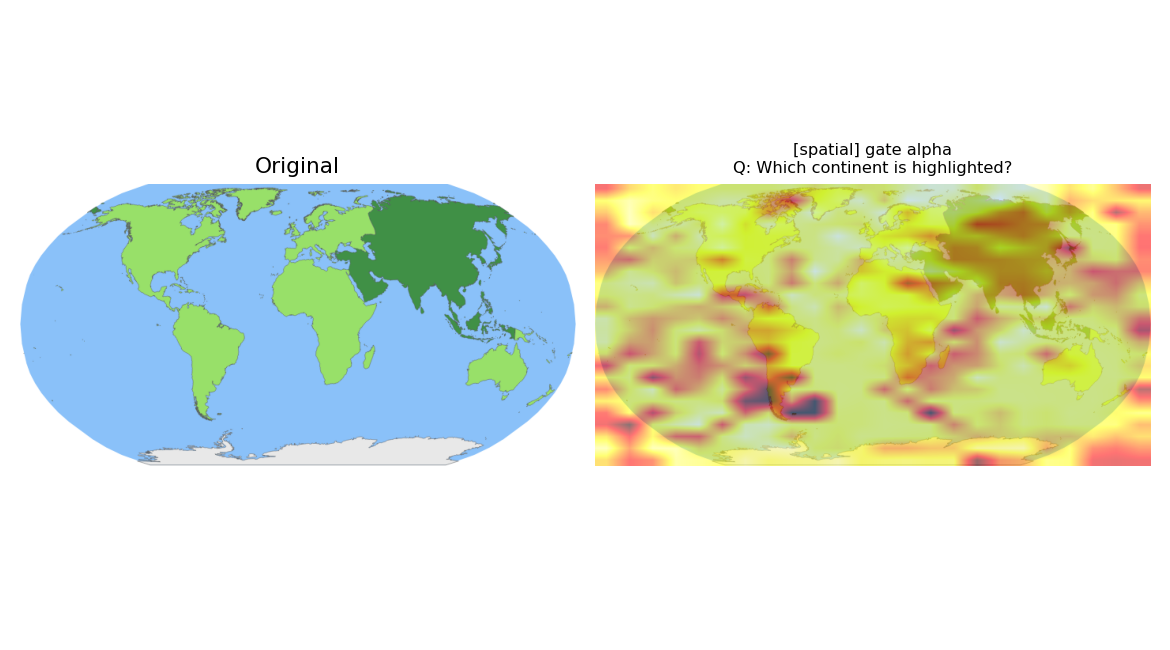
\includegraphics[width=\linewidth]{heatmap_spatial_1_idx15.png}
  \caption{``Which continent is highlighted?''}
\end{subfigure}
\hfill
\begin{subfigure}[b]{0.24\linewidth}
  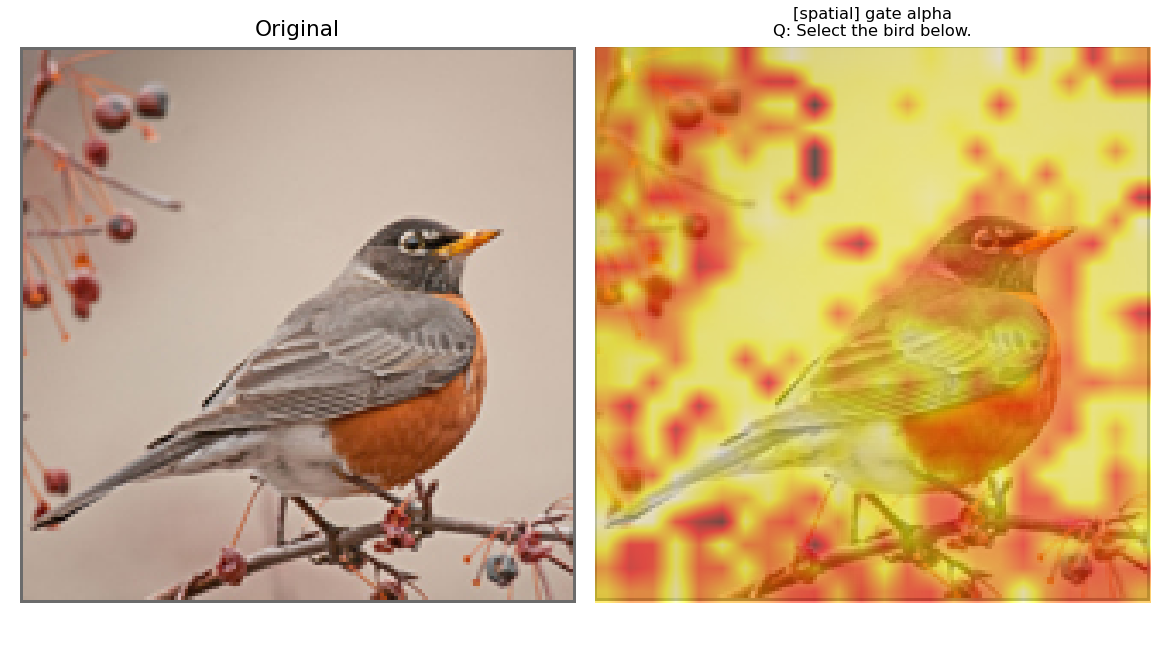
\includegraphics[width=\linewidth]{heatmap_spatial_2_idx18.png}
  \caption{``Select the bird below.''}
\end{subfigure}
\hfill
\begin{subfigure}[b]{0.24\linewidth}
  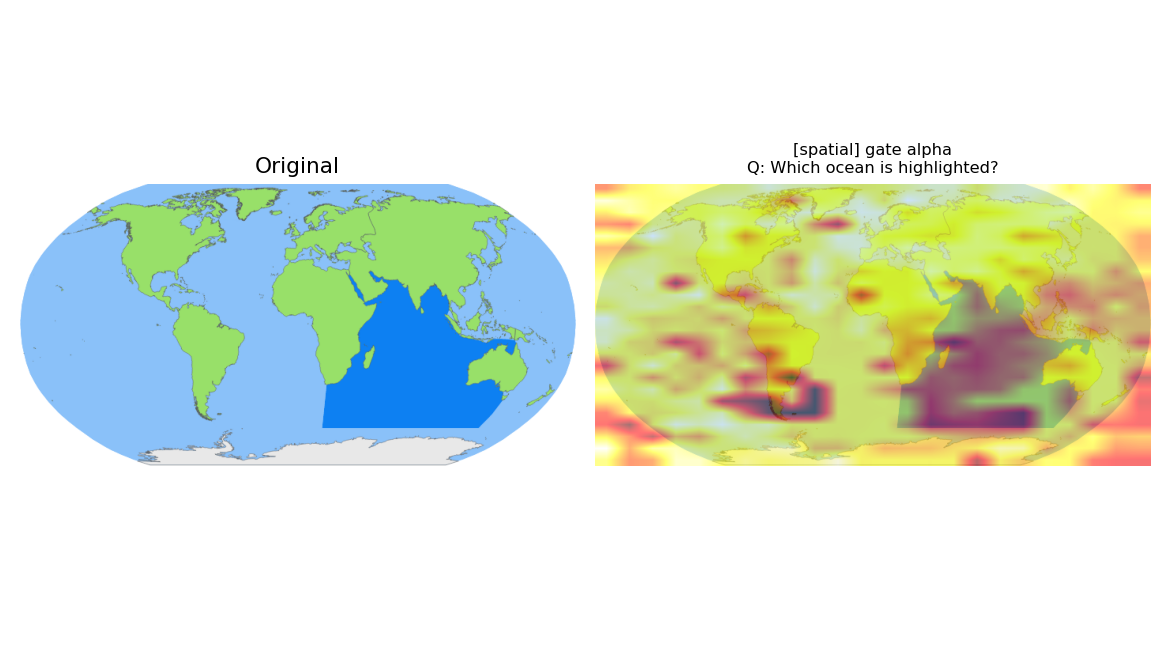
\includegraphics[width=\linewidth]{heatmap_spatial_3_idx28.png}
  \caption{``Which ocean is highlighted?''}
\end{subfigure}
\hfill
\begin{subfigure}[b]{0.24\linewidth}
  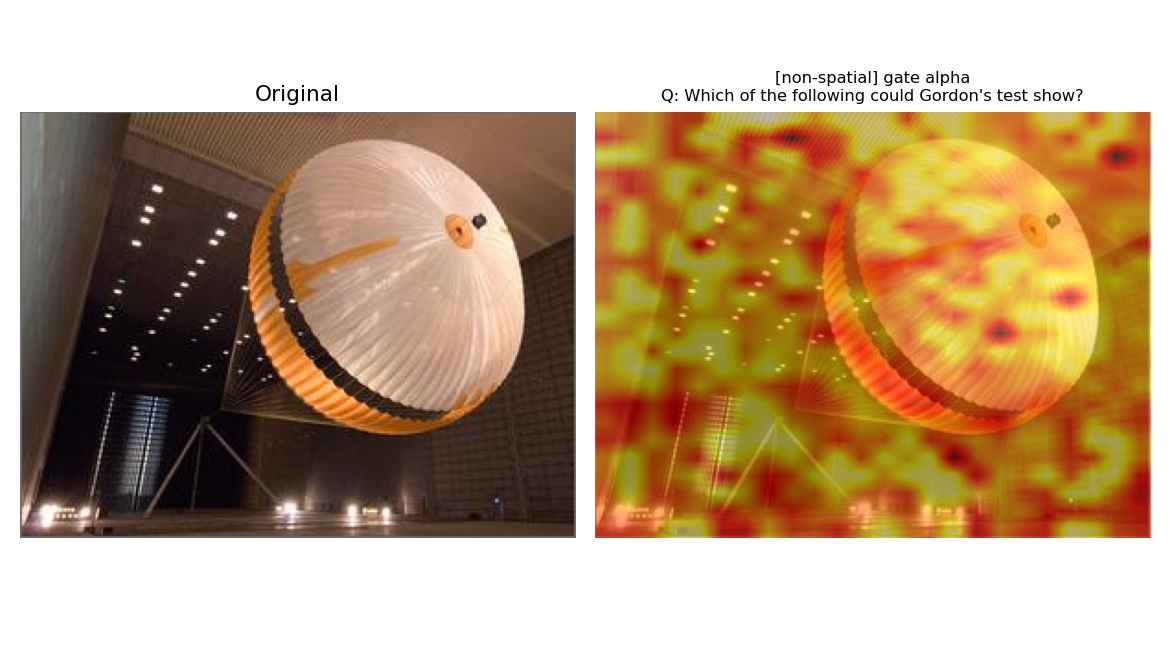
\includegraphics[width=\linewidth]{heatmap_counterexample_idx0.png}
  \caption{Counter-example: general question.}
\end{subfigure}
\caption{\textbf{QCGP gate weight heatmaps} ($\alpha_i$ overlaid on the source image; hot colours indicate higher patch relevance). Peak $\alpha$ values range 0.00199--0.00209 versus the uniform baseline $\approx0.00174$, consistent with $\tau_g \approx 1.0$ throughout training and indicating that QCGP has not acquired question-conditioned selectivity at this data scale.}
\label{fig:heatmaps}
\end{figure}

\subsection{Three-Bucket Failure Analysis}
\label{sec:failure}

We sample 100 errors uniformly at random (seed 42) from the 695 mistakes made by $E_1$ on the full 2{,}017-sample test split and classify each as a perception error (the model misread or ignored the image), a reasoning error (the image was read correctly but the wrong conclusion was drawn), or a CoT rescue (the error disappears when the prompt is re-issued with ``Let's think step by step''). The breakdown is 48\% perception, 41\% reasoning, and 11\% CoT rescue (Figure~\ref{fig:failure}). ScienceQA tests applied scientific knowledge rather than purely visual reading, so the larger reasoning fraction is consistent with the benchmark's design. The 11\% CoT-rescue fraction further indicates that a non-trivial share of apparent perception failures are actually inference-orchestration failures that would be addressed by chain-of-thought prompting rather than by a different connector.

\subsection{Subject-Level Accuracy}

Table~\ref{tab:subject} breaks down $E_1$'s full-test accuracy by ScienceQA subject. The aggregate $\Delta_v$ is $+5.0\%$, with natural science contributing the largest gap ($+5.1\%$) and language science the smallest ($+4.6\%$). The topic-level picture is more informative. Physics shows the largest topic-level $\Delta_v$ at $+14.1\%$, consistent with circuit and force-diagram questions whose answers cannot be inferred from the question text alone. Geography contributes 600 of the 2{,}017 test samples and reaches 78.3\% image accuracy with $\Delta_v = +7.7\%$. Economics is the only major subject with a strongly negative $\Delta_v$ ($-23.9\%$): text-only accuracy is 42.3\% versus 18.3\% with the image. Manual inspection indicates that the accompanying figures (typically supply-demand charts with embedded text) confuse rather than help the model. Biology shows a smaller negative $\Delta_v$ of $-2.0\%$, likely because biological diagrams require domain-specific structural knowledge that the model has not internalised at this scale.

\begin{table}[h]
\centering
\caption{\textbf{Subject-level breakdown for $E_1$} on the full 2{,}017-sample test split.}
\label{tab:subject}
\small
\begin{tabular}{lcccc}
\toprule
\textbf{Subject} & \textbf{N} & \textbf{Image Acc.} & \textbf{Text Acc.} & $\Delta_v$ \\
\midrule
Language Science & 44    & 70.5\% & 65.9\% & $+$4.6\% \\
Natural Science  & 1{,}209 & 62.7\% & 57.6\% & $+$5.1\% \\
Social Science   & 764   & 69.8\% & 65.1\% & $+$4.7\% \\
\midrule
\textbf{Overall} & \textbf{2{,}017} & \textbf{65.5\%} & \textbf{60.6\%} & \textbf{$+$5.0\%} \\
\bottomrule
\end{tabular}
\end{table}

\section{Discussion}
\label{sec:disc}

\paragraph{Pretrained Initialisation Dominates Architecture.}
The 30-point gap between $E_1$ and the random-init experts is the most decisive finding of our study. Because all four experts share training data, optimiser settings, and converge to similar final training loss, the gap cannot be attributed to optimisation difficulty or to inherent architectural weakness. It reflects the fact that $E_1$ enters fine-tuning with a projector that has already absorbed the geometry of CLIP-to-Vicuna translation over millions of image-text pairs, while $E_2$, $E_3$, and $E_4$ are asked to learn the same mapping from 6{,}218 samples. The practical implication is that any new connector architecture proposed for this regime must be warm-started from a pretrained projector if it is to compete on raw accuracy. Only the components that are genuinely novel relative to the LLaVA MLP, namely the Q-Former query vectors, the global pooling weights, and the QCGP gating layers, should remain randomly initialised.

\paragraph{MoC is Architecturally Viable but Overfits Quickly.}
The MoC's 73.8\% peak at epoch 2 demonstrates that the routing mechanism extracts a net benefit from heterogeneous experts even when three of the four are weaker individually than $E_1$. The 11.6-point fall to 62.2\% by epoch 5 and the inversion of $\Delta_v$ to $-8.0\%$ indicate that the system overfits to language patterns once the information available from the 6{,}218 training images is exhausted. Two factors plausibly contribute. First, the connector parameters reach a near-optimal solution around epoch 2 and subsequently drift toward configurations that interact poorly with LoRA adapters that continue to update. Second, MoE literature documents that routers can lock in suboptimal routing patterns once experts have specialised, and our load-balancing weight ($\lambda_{\text{lb}} = 0.01$) may be insufficient to re-equilibrate routing at later steps. Either way, validation-based early stopping is required; reproducing these results without it will substantially understate MoC's capacity.

\paragraph{QCGP Did Not Learn Selective Gating.}
QCGP did not acquire the per-question patch attention the architecture was designed for. The temperature $\tau_g$ remained within 0.0011 of its initialisation, and the heatmaps for spatially specific questions are statistically indistinguishable from those for the counter-example. The mechanism does function as a language-shortcut suppressor: $E_4$'s 13.0\% text-only accuracy is the lowest of any single configuration. The absence of question-conditioned selectivity, however, means that this suppression is not replaced by question-conditioned amplification of correct visual evidence. We attribute the failure to the same data scarcity that suppresses the other random-init experts: the bridging matrices $W_q$ and $W_k$ start from random initialisation, so the cosine similarities $\hat{u}^\top \hat{k}_i$ in Eq.~\ref{eq:qcgp} are essentially noise during the early training steps, and keeping $\tau_g \approx 1.0$ is the safe response to noisy similarities. If $W_q$ and $W_k$ were initialised from a projector that already aligns CLIP space with Vicuna space, the cosine signal would carry meaningful relevance information from the first step and $\tau_g$ would have an incentive to move.

\paragraph{Perception versus Reasoning on ScienceQA.}
The 48\%/41\%/11\% perception/reasoning/CoT-rescue distribution differs substantially from PAPO's 67\%-perception finding~\citep{wang2026papo}. The discrepancy reflects the benchmark difference: PAPO targets geometry-style problems where the image encodes most of the answer, whereas ScienceQA requires scientific knowledge in which the image is one of several inputs. MoC and similar connector-level interventions directly target the 48\% perception fraction. The 41\% reasoning fraction lies outside the connector's reach and would require either an explicit chain-of-thought objective or a dedicated reasoning module to address.

\subsection{Limitations}
\label{sec:limitations}

The main constraint of this study is the size of the training set relative to the number of newly introduced parameters. $E_2$, $E_3$, and $E_4$ add between 4M and 8.5M trainable parameters each but are trained on only 6{,}218 image-question pairs; this mismatch is the proximate cause of the random-init experts' underperformance and the near-stationary $\tau_g$. Pretraining on a larger image-text corpus before ScienceQA-specific fine-tuning would likely change both substantially. All QLoRA experiments were performed on a single A100 in Google Colab, where the effective batch size of 16, the choice of LoRA rank, and the number of epochs were each constrained by session-time and memory limits rather than by an exhaustive hyperparameter search. The router was trained jointly with the experts from initialisation, so early routing decisions were noisy and the load-balancing signal was correspondingly noisy during the most critical phase of training. Finally, because only the LoRA adapters were checkpointed, the trained router and QCGP parameters are not recoverable for post-hoc analysis on the full test split, which limits routing-behaviour claims to the training-time cumulative distribution.

\subsection{Future Work and Broader Implications}

Three follow-up directions emerge directly from the results. The most impactful is warm-starting $E_2$, $E_3$, and $E_4$ from $E_1$'s pretrained projector so that only their distinctive components (queries, pooling weights, gating layers) are learned from scratch. The second is staged training: freeze the experts at the best-validation checkpoint and continue training only the router, which would isolate whether the post-epoch-2 collapse is driven by expert drift or by router miscalibration. The third is to revisit QCGP under a curriculum in which $W_q$ and $W_k$ are trained on a contrastive image-text matching objective before joint fine-tuning, so that the cosine signal in Eq.~\ref{eq:qcgp} is informative from the first optimization step. 

\section{Conclusion}

This paper introduced the Mixture of Connectors, a question-conditioned routing system that selects among four structurally distinct connector experts and is trained jointly with a load-balancing objective. The full MoC reaches 73.8\% validation accuracy on the ScienceQA image-only split at epoch 2 and maintains a balanced expert distribution, demonstrating that routing across heterogeneous connectors is a practical architectural choice. The dominant empirical lesson concerns initialization rather than architecture: $E_1$'s 65.6\% versus 34--39\% for the random-init experts establishes that under a 6{,}218-sample budget, pretrained projector weights matter more than any single connector design choice. The MoC's overfitting past epoch 2 and the near-stationary QCGP temperature reinforce the same point from a different angle: the architecture has capacity that the training set is too small to fully exercise. Future progress on connector-level MoE in low-data regimes will therefore likely come from warm-starting heterogeneous experts from a shared pretrained projector and from staged training that decouples expert learning from router calibration.

\bibliographystyle{plainnat}
\bibliography{ref}

\end{document}
